\documentclass[aspectratio=169]{beamer}
\usetheme[block=fill]{metropolis}
\usepackage{tikz}
\usetikzlibrary{shapes.geometric, arrows.meta, positioning, calc}

\title{Building a Reproducible Scholarly Search Toolkit}
\subtitle{Episode 1: Reading the Contract}
\author{Scholar Search Kit}
\date{}

\begin{document}

\begin{frame}[plain]
  \titlepage
\end{frame}

\begin{frame}{What is an Architectural Contract?}
  \begin{itemize}
    \item Before writing a single line of code, we must define the \textbf{boundaries}.
    \item A contract specifies \textit{what} a component must do, not \textit{how} it does it.
    \item In this project, we read reference implementations to extract API signatures.
  \end{itemize}
  
  \vspace{0.5cm}
  \begin{center}
  \resizebox{\linewidth}{!}{
  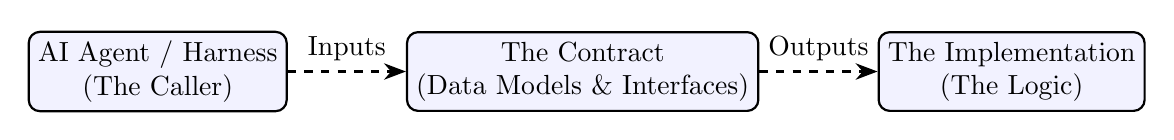
\begin{tikzpicture}[
      node distance=1.5cm,
      box/.style={rectangle, draw, thick, rounded corners, align=center, minimum width=3cm, minimum height=1cm, fill=blue!5},
      arrow/.style={-{Stealth[scale=1.2]}, thick, dashed}
    ]
    \node[box] (caller) {AI Agent / Harness\\(The Caller)};
    \node[box, right=of caller] (contract) {The Contract\\(Data Models \& Interfaces)};
    \node[box, right=of contract] (impl) {The Implementation\\(The Logic)};

    \draw[arrow] (caller) -- node[above] {Inputs} (contract);
    \draw[arrow] (contract) -- node[above] {Outputs} (impl);
  \end{tikzpicture}
  }
  \end{center}
\end{frame}

\begin{frame}{The Master Component Specifications}
  We have compiled our extracted contracts into \texttt{docs/component-specs.md}.
  
  \vspace{0.3cm}
  \textbf{Status Tiers:}
  \begin{itemize}
    \item \textcolor{green}{[Baseline v0.1.0]} - Currently active and tested.
    \item \textcolor{orange}{[Lesson Milestone Target]} - What we will build together.
    \item \textcolor{blue}{[Reference Architecture]} - External inspiration.
  \end{itemize}
\end{frame}

\begin{frame}{The 8-Step AI Build Loop}
  To build this toolkit safely with AI, we enforce an 8-step protocol for every lesson:
  \begin{enumerate}
    \item Scientific Need \& Context
    \item Reference Architecture Reading
    \item Explicit Contracts
    \item Edge Cases \& Counterexamples
    \item Build Request (Prompt)
    \item Proof (Tests)
    \item Human Review
    \item Status Record
  \end{enumerate}
\end{frame}

\begin{frame}{Why not just prompt for the whole thing?}
  \begin{alertblock}{The Hallucination Trap}
    Asking an AI to "build a literature review tool" results in monolithic, tightly-coupled, untestable code.
  \end{alertblock}
  
  \vspace{0.3cm}
  By providing strict boundaries (the contracts) and writing tests first, we constrain the AI to act as a highly skilled typist rather than a rogue architect.
\end{frame}

\begin{frame}[standout]
  Next up: Package Architecture \& Scaffolding
\end{frame}

\end{document}
